% Current dataset/metric specification: 25 October 2026. Unmeasured results stay blank.
\documentclass[10pt,twocolumn,letterpaper]{article}
\usepackage[review]{cvpr}
\usepackage{times,graphicx,amsmath,amssymb,booktabs,tabularx,multirow,xspace}
\usepackage[T1]{fontenc}
\usepackage{microtype}
\clubpenalty=10000
\widowpenalty=10000
\definecolor{cvprblue}{rgb}{0.13,0.40,0.67}
\usepackage[pagebackref,breaklinks,colorlinks,allcolors=cvprblue]{hyperref}
\def\paperID{Draft}
\def\confName{CVPR}
\def\confYear{2027}
\newcommand{\ours}{\textup{\textsc{BrickPlan}}\xspace}
\newcommand{\sig}{\sigma}
\title{BrickPlan: A Benchmark for Visual Assembly and Error Recovery}
\author{Anonymous submission}
\begin{document}
\makeatletter
\twocolumn[{
\begin{@twocolumnfalse}
\maketitle
\centering
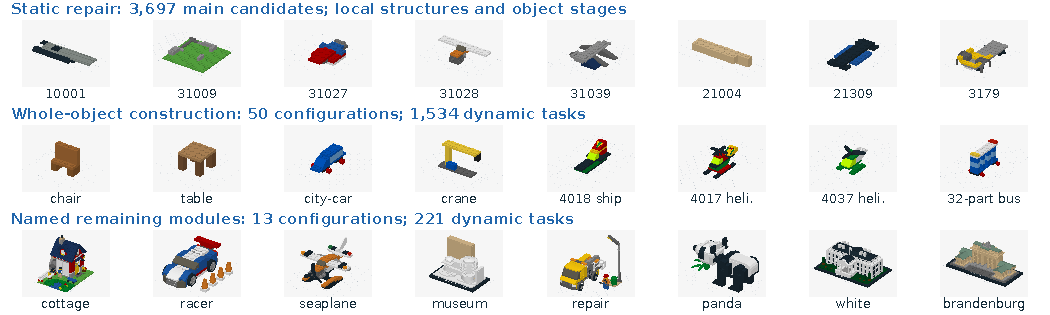
\includegraphics[width=\textwidth]{figures-current/teaser.pdf}
\captionof{figure}{\textbf{Repair a supplied state or keep building through an unexpected change.} The collection has 5,720 distinct task records. Its 5,452 main candidates comprise 3,697 static tasks and 1,755 dynamic tasks; 268 historical dynamic structure/crop tasks remain diagnostic only. Dynamic object tasks cover 50 whole-object and 13 named-module configurations. Small original LDraw objects retain every source part; larger objects supply the surrounding assembly.}
\label{fig:teaser}
\vspace{10pt}
\end{@twocolumnfalse}
}]
\makeatother

\begin{abstract}
Visual assembly requires an agent to maintain a correct structure while
its own actions and unexpected changes alter the scene. We introduce
\ours, a benchmark for static repair and continuous construction with
hidden interventions. The organized collection contains 5,720 distinct
tasks, including 5,452 main candidates spanning local static structures,
complete objects, and named remaining modules. Dynamic tasks cover
63 operation configurations and include 43 episodes with two or three
interventions. Seven physical error labels are distinguished from
access-related process errors and intervention counts. Agents inspect
actual RGB states and execute one brick action at a time; acceptance
compares terminal geometry, color, and part type, allowing different
legal construction orders. We define static correction and damage
metrics, and dynamic recovery metrics with explicit control, exposure,
and event-effect requirements. All 5,922 retained execution conditions
pass reference replay, while a historical route diagnostic shows that
reference-prefix triggers miss opportunities on valid alternative
routes. These are executor checks, not learned-agent results. We provide
named model candidates and unmeasured experiment tables; current-interface
human qualification and formal model evaluation remain outstanding.
\end{abstract}

\section{Introduction}
An agent assembling a toy car may build the left side before the right,
while another follows the opposite order. Both can finish correctly.
An evaluator that compares every intermediate state with one manual
would reject a valid route. Scheduling an accident only when an agent
reproduces that same reference prefix creates a second problem: a
correct alternative route may never encounter the accident. A benchmark
must separate the final structure, physical action legality, and actual
exposure to a fault.

The visual specification also matters. A final image can hide joints or
internal pieces, making reconstruction ambiguous even for a person.
We therefore distinguish local static repair from dynamic construction
of recognizable objects. Small community models are built in full;
large scenes supply an already assembled body and ask the agent to
complete an identifiable roof, cabin, or tail. Available manuals describe
one feasible route. They establish intended structure without imposing
that route as the only acceptable sequence.

\ours connects these settings through a common interaction contract.
A static task supplies an imperfect state and one stage target. A dynamic
task supplies a fixed whole-object or module target, then allows uninterrupted
inspection and one-brick operations. Hidden interventions can remove,
replace, move, or add pieces after progress has been made. The agent
must finish the task through ordinary actions, without a forced
mid-episode declaration that an error occurred.

Prior work addresses buildable generation~\cite{pun2025brickgpt,kulits2026bricknet},
manual execution~\cite{wang2022mepnet}, assembly-step
correction~\cite{wan2024scanet}, and interactive structural
understanding~\cite{walsman2022breakmake}. Agentic design and robot
recovery further motivate robust evaluation~\cite{kulits2026brickbench,li2026roborecover}.
Our contribution is the task and measurement contract linking visual
history, legal alternative orders, and externally altered ongoing work.

\paragraph{Contributions.}
(1) We organize 5,720 distinct tasks with explicit scope, source grouping,
error labels, and structural grades; 5,452 are main candidates.
(2) We define a shared visual action interface and terminal scoring
that accepts interchangeable parts and alternative legal orders.
(3) We separate correction from damage, and raw completion from qualified
recovery, including repeated interventions and technical censoring.
Reference replays and route diagnostics support these protocol claims.
Formal model rankings and human performance are not yet established.

\begin{figure}[t]
\centering
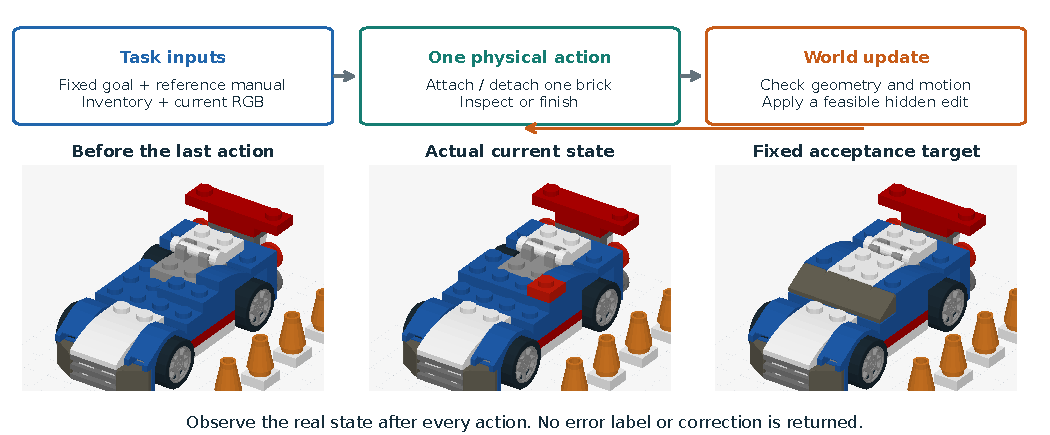
\includegraphics[width=\linewidth]{figures-v2/protocol.pdf}
\caption{\textbf{Continuous interaction.} One target remains available. Each action is checked; the next observation shows the actual state after execution and any hidden intervention. An error label or correction is never supplied. Manuals are queried where supported.}
\label{fig:protocol}
\end{figure}

\section{Related Work}
\paragraph{Brick generation and visual assembly.}
BrickGPT generates buildable structures using validity filtering and
rollback~\cite{pun2025brickgpt}; BrickNet models connector graphs and
assembly sequences from human-designed LDraw objects~\cite{kulits2026bricknet}.
BrickBench evaluates agentic design under validity, alignment, and
quality criteria~\cite{kulits2026brickbench}. We reuse brick geometry and
connection infrastructure rather than claim a new physics simulator.
Our goal is specified in advance, so correctness is restoration or
completion of that goal rather than open-ended design quality.

Break and Make combines inspection, disassembly, and
reconstruction~\cite{walsman2022breakmake}. LEGO-Puzzles and PhyBlock
study spatial reasoning, planning, and physical understanding through
block tasks~\cite{tang2025legopuzzles,ma2025phyblock}. MEPNet executes
visual manuals~\cite{wang2022mepnet}; LEGO-ECA and SCANet address errors
and corrections associated with assembly steps~\cite{wan2024scanet}.
These are close to our static condition. Our dynamic condition retains
the agent's ongoing history across an external change and permits
inspection, repair, and further construction in the same episode.

\paragraph{Adaptation and recovery.}
AsgardBench evaluates visually grounded plan adaptation with lightweight
feedback~\cite{tupini2026asgard}; RoboRecover evaluates continuation from
execution deviations~\cite{li2026roborecover}. Recovery itself is therefore
not novel. Our distinction is instruction-assisted brick construction
with one-part execution, alternative-order acceptance, and recovery
eligibility conditioned on what actually happened. We adapt part-quality
and correction/damage analysis~\cite{walsman2022breakmake,wan2024scanet},
while defining metrics for our own action and observation contract.

\section{Dataset Construction and Organization}
\subsection{Counting tasks, conditions, and objects}
Table~\ref{tab:dataset} separates task scopes. The catalogue contains
5,839 records: 5,793 earlier records plus 46 conditions for three complete
LDraw objects. Within the same source, configuration, and task contract,
physical equivalence identifies 119 repeated records: 27 static problems
and 92 normal dynamic controls. Deduplication leaves 5,720 distinct tasks.
This is not a claim of global semantic deduplication across different sources.
An additional 83 cross-adapter aliases remain execution conditions, not
new catalogue tasks. Thus 5,922 conditions are retained for replay.

The main candidate set contains 3,697 static and 1,755 dynamic tasks.
Static local fragments remain useful for structure repair. In contrast,
224 historical dynamic mechanism tasks and 44 arbitrary-crop dynamic
tasks are excluded from object-construction conclusions. They remain
available as separate diagnostics. ``Candidate'' denotes program-checked
content; it does not certify that every image has passed independent
human qualification.

\begin{table*}[t]
\centering\small
\caption{\textbf{Current dataset after within-contract deduplication.} Controls are included. Main candidates sum to 5,452; the two diagnostic rows add 268. Configuration counts and task counts are different units, and source objects overlap across static and dynamic tasks.}
\label{tab:dataset}
\begin{tabularx}{\textwidth}{@{}lrrX@{}}
\toprule
Task scope & Distinct tasks & Main & Start and acceptance target\\
\midrule
Local static structure & 3,315 & Yes & Supplied local state $\to$ its required stage.\\
Whole-object static stage & 148 & Yes & Supplied whole-object stage $\to$ stage target.\\
Named-module static stage & 234 & Yes & Supplied body and module state $\to$ stage target.\\
Whole-object dynamic & 1,534 & Yes & Empty white plate $\to$ complete object (50 configurations).\\
Named-module dynamic & 221 & Yes & Supplied body $\to$ completed named module (13 configurations).\\
Historical dynamic structure & 224 & No & Structural execution and recovery diagnostics.\\
Archived arbitrary-crop dynamic & 44 & No & Traceability only; excluded from object main results.\\
\midrule
Total & 5,720 & 5,452 & 3,697 main static tasks and 1,755 main dynamic tasks.\\
\bottomrule
\end{tabularx}
\end{table*}

\subsection{Recognizable objects and retained coverage}
The 63 primary dynamic configurations comprise 50 whole-object builds
and 13 named-module builds. Whole objects include all 42 earlier
procedural designs, five longer procedural objects, and three complete
original LDraw models. The latter are a 12-part ship (4018), a 13-part
sea helicopter (4017), and a nine-part helicopter (4037). Their downloaded
source files retain every part, color, and transform; none is removed to
simplify the task. This certifies source-file coverage, not a retail-set
bill of materials. The five longer builds contain 21--32 active parts.

Named modules come from twelve community source scenes, with an additional
expanded museum-roof configuration. Their surrounding scene is supplied
as immutable context. These are thirteen operation configurations, not
thirteen new source sets. Earlier chairs, tables, cars, and machines
remain in the suite. The supplement illustrates all dynamic configurations
and enumerates all 160 configurations in the original static bank.

\subsection{Errors, process demands, and structural grades}
Seven basic labels describe physical discrepancies: missing, extra,
wrong color, wrong part, displaced position/height, non-equivalent
orientation, and swapped positional relations. Labels may co-occur.
Part substitutions include size and thickness; local extra layers are
extra-piece proxies, not whole-model layer duplication.

Process tags describe premature covering and buried repair, rather
than adding more mutually exclusive physical classes. A buried color
error can carry both the color and buried-repair labels. Multiple
simultaneous defects differ from multiple temporally separated accidents.
The 43 main repeated-event tasks contain 37 two-event and six three-event
conditions. Community-inspired human-error tags cover twelve approved
source categories; they describe synthetic analogues, not measured
frequencies or collected human mistake trajectories.

\begin{table}[t]
\centering\small
\caption{\textbf{Physical error coverage in main candidates.} S: static; W/M: whole/module dynamic. Labels co-occur; rows do not sum to task totals. Module swap is an explicit coverage gap.}
\label{tab:labelcoverage}
\begin{tabularx}{\linewidth}{@{}Xrrr@{}}
\toprule
Physical label & S & W & M\\
\midrule
E01 Missing & 1,361 & 209 & 60\\
E02 Extra & 356 & 167 & 36\\
E03 Color & 1,458 & 426 & 60\\
E04 Part & 339 & 185 & 15\\
E05 Position & 804 & 227 & 32\\
E06 Orientation & 489 & 130 & 25\\
E07 Swap & 31 & 20 & 0\\
\bottomrule
\end{tabularx}
\end{table}

We use separate structural descriptors. Build length is B1 ($\leq12$),
B2 (13--24), or B3 ($\geq25$) active target pieces. Static length counts
only its acceptance stage. Rework is R0 for controls; R1 for a reference
repair of at most two moves without removing correct covers; R2 for
remaining ordinary/multiple-defect repair; and R3 when the witness removes
correct covers or uses at least seven moves. These are feasible-witness
burdens, not proven minimum requirements. T0--T3 count external events;
all static tasks are T0. Visibility is recorded independently.
Planning grades G1/G2/G3 combine these descriptors and contain
2,577/2,823/52 main candidates. They are not empirically validated
``easy/medium/hard'' labels. The supplement gives the exact rules.

\begin{figure*}[t]
\centering
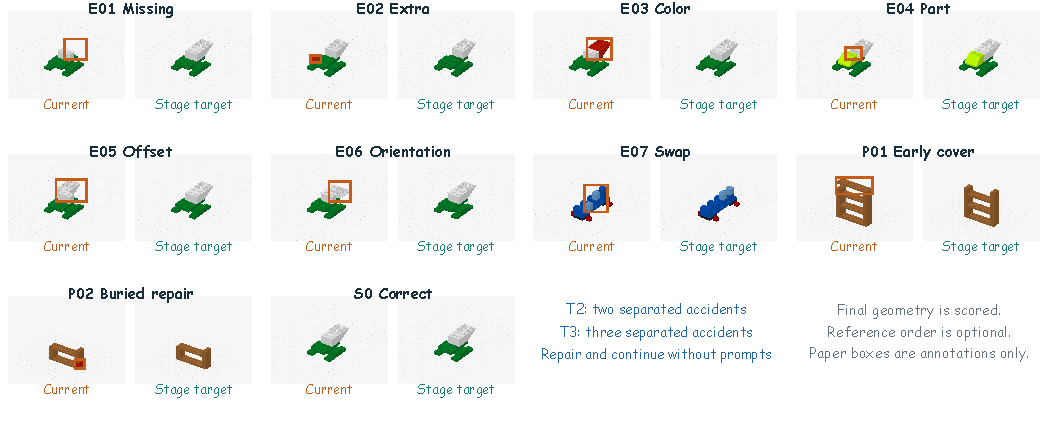
\includegraphics[width=\textwidth]{figures-current/errors.pdf}
\caption{\textbf{Seven physical error labels, two process burdens, and a correct control.} Each pair shows an actual current state and its sole stage target with matched framing. Small helicopter examples use the required intermediate stage, not the completed nine-part object. E07 uses the longer bus; P01/P02 use the bookshelf. Orange boxes highlight pixel differences for the paper only. Simultaneous errors and temporally repeated events are different annotations.}
\label{fig:errors}
\end{figure*}

\section{Observation and Execution Contract}
\subsection{One acceptance target and one action object}
A task has fixed context $B$, movable inventory $P$, finite pose candidates
$C_p$, initial state $s_0$, and target $g$. A part is installed at one
candidate or remains on the rack. All tasks use a fixed construction
coordinate frame and white-baseplate environment; module tasks also
retain a preassembled body that cannot be manipulated.

The current input version uses actual RGB scenes, neutral instructions,
and anonymous part/position handles. It supplies one acceptance target:
a stage target for static tasks, or the complete required object/module
for dynamic tasks. Future manual pages are references, never additional
acceptance goals. Isometric, rear, and top inspection are available.
Current and target comparison panels each use an $800\times600$ scene
on the same $1600\times636$ canvas. Full-object context remains visible
for named modules. Manuals are queryable in community, expanded, and
complete-LDraw tasks; legacy local static tasks have no step manual.
Different information conditions are reported separately.

The response is one direct JSON action object, with no track-specific
outer wrapper:
\begin{equation}
 a_t\in\{\operatorname{attach}(p,c),\operatorname{detach}(p),
          \operatorname{inspect}(q),\operatorname{finish}\}.
\end{equation}
Each manipulation moves one brick. Inspections query a supported view,
part, candidate preview, or manual page. A preview is hypothetical and
neither installs a part nor marks it as correct. The public observation
excludes task family, hidden states, event schedule, and reference actions.
Inventory is a part catalogue with spares, not a live remaining-piece oracle.

\begin{figure*}[t]
\centering
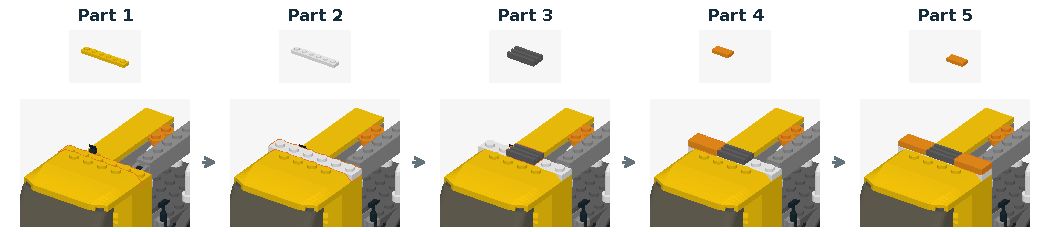
\includegraphics[width=\textwidth]{figures-v2/instructions.pdf}
\caption{\textbf{Seven-part manual as one feasible route.} Each column shows one physical part and the resulting reference state. The seaplane body is supplied. Orange outlines explain the added part in the manual; ordinary current-state images do not highlight errors. These publication crops explain the module and do not replace the full-context evaluation views.}
\label{fig:manual}
\end{figure*}

\subsection{Legality and order-independent completion}
An attachment must have a valid pose, a supported compatible connection,
no endpoint collision, and a clear straight insertion path. Detachment
checks a straight extraction path. Rejected attempts leave the scene
unchanged and return a legality code. They consume the declared attempt
budget, but do not prevent later success. Rigid pose/connection checks
do not simulate force, slipping, flexible joints, or a gripper.

Let $\sig(s)$ be the multiset of installed shape, color, and pose records,
using only supported symmetry equivalences. Completion requires
\begin{equation}
 C(\tau)=\mathbf{1}[a_T=\operatorname{finish}]
          \mathbf{1}[\sig(s_T)=\sig(g)].
 \label{eq:completion}
\end{equation}
Interchangeable same-shape, same-color pieces are not distinguished by
internal ID. Asymmetric or decorated parts are not granted arbitrary
rotational equivalence. The immutable body is excluded from part scores;
adding ten roof pieces must not receive credit for 500 supplied wall
pieces. No arbitrary global registration is applied. Floating pieces,
duplicates, collisions, or state replacement cannot bypass execution.

A manual supplies one verified witness, not mandatory intermediate states.
Two legal prefixes can have equal progress and different geometry
(Fig.~\ref{fig:orders}). Static repair ends at its stated stage even when
later manual pages describe the finished object.

\begin{figure}[t]
\centering
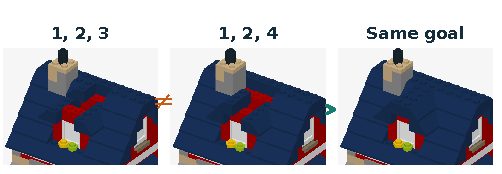
\includegraphics[width=\linewidth]{figures-v2/alternative-orders.pdf}
\caption{\textbf{Different legal prefixes, same goal.} These roof routes differ after three placements. Reference indices identify intended placements, not compulsory action times. Both routes are accepted by terminal scoring.}
\label{fig:orders}
\end{figure}

\subsection{Interventions and visual qualification}
Hidden edits occur between observations after accepted manipulations.
The executor logs their actual timing, location, and legal primitives.
Adaptive module selectors search the actual installed state; some older
conditions use template-dependent opportunities. Neither a scheduled
fault nor a nominal step threshold proves exposure. An infeasible event
is deferred or untriggered. Multi-event tasks record every occurrence;
one of two planned accidents is only partial exposure.

All 5,922 retained conditions pass fresh legal reference replay, with
zero failures. This establishes witnessed feasibility, not visual
understanding. The three complete LDraw objects have 46 checked
conditions: 36 reference fault images exceed 128 changed pixels at
24 intensity levels in at least one native view, and ten are controls.
Adaptive locations require their own check. Older cropped module pixel
checks do not certify the new full-context views. Complete current-interface
image admission and independent human review remain pending. Low contrast
and an event that cancels the latest action are flagged separately;
absence of an obvious before/after change is not proof of a model miss.

\section{Evaluation Metrics}
\subsection{Static correction and collateral damage}
We distinguish S0 (260 correct-stage acceptance tasks) and S1 (3,437
repair tasks). Let $I,F,G$ be the initial, final, and goal movable-part
multisets and $H=I\cap G$ the initially correct placements. Exact SR is
Eq.~\ref{eq:completion} averaged over valid S1 runs. Partial quality and
repair progress are
\begin{align}
 \mathrm{F1}_{\rm place}&=\frac{2|F\cap G|}{|F|+|G|},\\
 d(A,G)&=|A-G|+|G-A|,\\
 \mathrm{ER}&=1-\frac{d(F,G)}{d(I,G)},\qquad
 \mathrm{DR}=\frac{|H-F|}{|H|}.
\end{align}
ER can be negative. A wrong-color substitution contributes one missing
correct placement and one excess placement; residual count is neither
human error count nor minimum action cost. Temporarily dismantling then
restoring a correct cover causes no terminal DR. On S0, false repair
(FR) records any accepted attach/detach, even if the agent later restores
the target. S0 accuracy and S1 SR are not pooled. Undefined denominators
are N/A; F1 of two empty multisets is one. Attribute-combination F1,
original missing recovery, and original excess clearance are supplemental.

\begin{table*}[!ht]
\centering\small
\caption{\textbf{E1: static repair (unmeasured).} Implemented. Separate whole-object and finishing stages; SR/F1/ER/DR use S1 and FR uses S0. Dashes mean not run, never zero.}
\begin{tabularx}{\textwidth}{@{}Xrrrrrr@{}}\toprule
Model & SR & F1 & ER & DR & S0 FR & Valid N\\\midrule
GPT-6.1 Sol & --- & --- & --- & --- & --- & ---\\
Claude Sonnet 5.5 & --- & --- & --- & --- & --- & ---\\
Gemini 3.8 Flash & --- & --- & --- & --- & --- & ---\\
Claude Haiku 5.5 & --- & --- & --- & --- & --- & ---\\
Qwen3.5-9B & --- & --- & --- & --- & --- & ---\\
Qwen3.5-27B & --- & --- & --- & --- & --- & ---\\
InternVL3.5-8B & --- & --- & --- & --- & --- & ---\\
Qwen2.5-VL-7B & --- & --- & --- & --- & --- & ---\\
Qwen2.5-VL-32B & --- & --- & --- & --- & --- & ---\\
Gemma 3-12B & --- & --- & --- & --- & --- & ---\\
\bottomrule
\end{tabularx}
\end{table*}


\subsection{Dynamic construction, exposure, and qualified recovery}
D0 has 63 normal builds; D1 has 1,649 single-event tasks; D2 has 43
repeated-event tasks. BCR is normal-build completion and ICR is raw
completion of valid intervention-assigned runs, including untriggered
runs. Trigger rate TR counts actual events over planned events.
Neither ICR nor TR is detection accuracy.

For causal comparisons, save a common environment/conversation prefix
and branch it into control and intervention continuations. Both branches
retain the same prior images, handle mapping, used budget, and settings.
Let $Q$ contain pairs with valid branches, a verified shared prefix,
all planned events triggered, and verified incident effects. An edit
that removes the agent's already-wrong piece cannot automatically earn
repair credit. An early correct cover requires evidence that it blocks
future access rather than an increase in terminal residual alone.
For control/fault outcomes $c_i,f_i$, define
\begin{equation}
 \mathrm{CRR}=\frac{\sum_{i\in Q}c_i f_i}{\sum_{i\in Q}c_i},\qquad
 \Delta\mathrm{SR}=\frac{1}{|Q|}\sum_{i\in Q}(c_i-f_i).
 \label{eq:recovery}
\end{equation}
CRR conditions on successful normal construction; the signed paired
difference does not. Report planned/valid pairs, failed controls,
untriggered/partial-event pairs, verified effects, and eligible $N$.
Unreached faults are not repair failures or missed detections.

\begin{table*}[t]
\centering\small
\caption{\textbf{E2: dynamic construction and recovery (unmeasured).}  W/M: whole-object/named-module scope. BCR uses D0; CRR requires normal success and verified complete exposure; $\Delta$ uses eligible pairs without filtering control success. Report D1 and D2 separately. ICR, TR and eligibility counts are retained in E3/E6/E9 and the ledger.}
\label{tab:dynamic-main}
\begin{tabularx}{\textwidth}{@{}Xrrrrrr@{}}
\toprule
Model & W BCR & W CRR & W $\Delta$ & M BCR & M CRR & M $\Delta$\\
\midrule
GPT-6.1 Sol & --- & --- & --- & --- & --- & ---\\
Claude Sonnet 5.5 & --- & --- & --- & --- & --- & ---\\
Gemini 3.8 Flash & --- & --- & --- & --- & --- & ---\\
Claude Haiku 5.5 & --- & --- & --- & --- & --- & ---\\
Qwen3.5-9B & --- & --- & --- & --- & --- & ---\\
Qwen3.5-27B & --- & --- & --- & --- & --- & ---\\
InternVL3.5-8B & --- & --- & --- & --- & --- & ---\\
Qwen2.5-VL-7B & --- & --- & --- & --- & --- & ---\\
Qwen2.5-VL-32B & --- & --- & --- & --- & --- & ---\\
Gemma 3-12B & --- & --- & --- & --- & --- & ---\\
\bottomrule
\end{tabularx}
\end{table*}


\paragraph{Recovery while continuing to build.}
For event states $B$ before and $A$ after, event-specific obligations are
lost correct placements $L=(B\cap G)-A$ and incremental excess
$X=(A-G)-(B-G)$. A later state repairs these quantities without having
to equal $B$; correct additional progress is allowed. The window ends
before the next external event. Record first recovery in decisions,
window-end recovery, and retention over at least two subsequent
decisions. Observed regression fails retention; an otherwise correct
short window is N/A. Process-only obstruction with empty $L,X$ receives
no automatic zero-latency recovery. Repair@$k$ ($k=2,4,8$) is reserved
for sufficiently observed single-event or checkpoint trials.

\paragraph{Failures, aggregation, and missing data.}
Premature finish and model decision-budget exhaustion are ability failures.
Final service errors, harness errors, and external stops are censored
from ability rates and listed separately. A transient error that recovers
within the same decision does not censor a completed run; its cost remains.
Report valid coverage and completion per planned attempt alongside
ability scores. Parsing, schema/ID errors, and physical rejections have
separate counters. Legal-action rate uses well-formed manipulation
attempts. Action cost is relative to a feasible witness, not SPL or
proven optimal efficiency.

Normalize aliases, average within object, and report object- and
source-macro estimates plus task-micro references. Separate input version,
track, and task type. Error rows are multilabel; their counts do not add
to a dataset size. Future 95\% intervals resample source groups, not
nominally independent variants. The current 154 groups have zero
cross-split overlap; 45 displayed/debugged sources are public development.
There is no untouched new-source community test in this release.

\section{Diagnostics and Experiment Design}
\subsection{Reference replay and route sensitivity}
The current replay audit covers 3,292 S, 1,712 D, 96 M, 776 expanded,
and 46 original-object conditions, including aliases. These are legal
reference executions, not model scores. A separate historical diagnostic
uses twelve modules, two verified routes, and four conditions per route:
96 route--condition trials. Exact-prefix opportunities on alternative
routes occur in 9/36 fault trials, versus 36/36 actual-state events
(Table~\ref{tab:diagnostic}). Alternative routes were selected as regression
counterexamples, not sampled from agent behavior. The blind continuation
finishes 24/24 controls and 0/72 faults; a privileged inverse-based
recovery finishes 96/96. Both are scripts. These historical numbers do
not establish current-suite visual or model performance.

\begin{table}[t]
\centering\small
\caption{\textbf{Historical route diagnostic.} All normal routes are legal and finish. Fault denominators are three families per module. No learned model is involved.}
\label{tab:diagnostic}
\begin{tabularx}{\linewidth}{@{}Xrr@{}}
\toprule
Check & Reference & Alternative\\
\midrule
Normal terminal geometry & 12/12 & 12/12\\
Every prefix matches manual & 12/12 & 0/12\\
Exact-prefix opportunity & 36/36 & 9/36\\
Actual-state event & 36/36 & 36/36\\
\bottomrule
\end{tabularx}
\end{table}

\begin{figure*}[t]
\centering
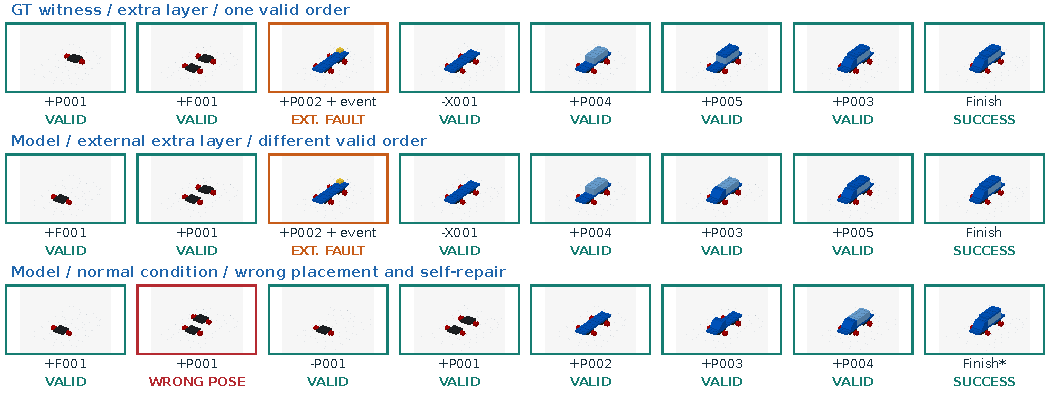
\includegraphics[width=\textwidth]{figures-v2/repair-comparison.pdf}
\caption{\textbf{Reference and archived model repair, eight states per row.} Top: one feasible GT witness. Middle: an archived Gemini 4 Argon rollout repairs an extra-layer event using another legal order. Bottom: a separate normal rollout corrects its own legal but wrong placement. All three eventually succeed. Green/orange/red indicate valid state/external change/wrong placement. $+$/$-$ mean attach/detach; * omits intervening operations. The 32 model decisions replay exactly. These v5 examples are historical development illustrations, not current scores or shared-prefix pairs.}
\label{fig:repair}
\end{figure*}

\subsection{Planned model, human, and input comparisons}
Tables~\ref{tab:static-main}--\ref{tab:dynamic-main} retain ten previously
selected candidates: four API models and six open visual models,
including Qwen2.5-VL and Gemma 3. The roster is a planned comparison;
exact served revisions, image support, and account access must be checked
before execution. Each model/condition runs once, with seed 41 for
handle randomization. The candidate pool and audited test assignments
are specified in the supplement. No old 467-question or 168-fault sample
is silently reused as the current unified test split. The current
existing-source test contains 392 main candidates: 309 local-static
and 83 whole-object dynamic tasks. Public module and original-object
results remain development analyses. Longer-community, repeated-event,
and untouched-source coverage should be evaluated separately, with
admission and eligibility counts for each claim.

All compared models receive the same declared task list, information,
and budgets within a track. A proposed outer cap is $\max(40,6N+20)$
decisions, including inspection and malformed replies, while applicable
native manipulation caps remain recorded. These proposed comparison
settings are not a claim that every API adapter is already connected.
Store every request, image hash/dimension, reply, accepted action,
termination status, event, token use, and charge. Actual budgets and
costs must come from a current-interface pilot, not old car prices.

\begin{table}[t]
\centering\small
\caption{\textbf{E3: input ablations (unmeasured).} Each cell reports D/M recovery; use identical cases and seeds. Sol = GPT-6.1 Sol; Argon = Gemini 4 Argon; Qwen = Qwen3.5-27B. M-only manual ablation has no D value. Symbolic input is privileged.}
\label{tab:ablations}
\begin{tabularx}{\linewidth}{@{}Xrrr@{}}
\toprule
Input condition & Sol & Argon & Qwen\\
\midrule
Full visual interface & --- & --- & ---\\
No previous image & --- & --- & ---\\
No manual (M only) & n/a / --- & n/a / --- & n/a / ---\\
No candidate preview & --- & --- & ---\\
Success/failure feedback & --- & --- & ---\\
Symbolic state & --- & --- & ---\\
\bottomrule
\end{tabularx}
\end{table}


\begin{figure}[t]
\centering
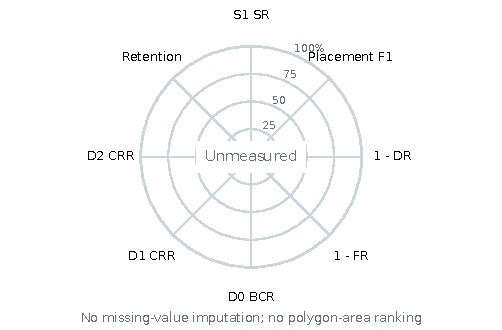
\includegraphics[width=\columnwidth]{figures-current/evaluation-radar.pdf}
\caption{\textbf{Metric profile template, unmeasured.} Axes expose distinct outcomes; $1-\mathrm{DR}$ and $1-\mathrm{FR}$ reverse the two lower-is-better rates. No model curve, missing-value imputation, or polygon-area score is used. Track, counts, and uncertainty remain in tables.}
\label{fig:radar}
\end{figure}

The default condition is RGB with neutral task text and action handles,
not pure image input. Text-state and RGB-plus-state conditions are planned
separately: explicit poses can expose occluded geometry and are privileged
relative to RGB. Free coordinates add localization burden and require a
separate output experiment. Manual/history/view/feedback changes each
hold the other factors fixed. Input changes require fresh paired prefixes
and visibility checks.

\begin{table}[t]
\centering\small
\caption{\textbf{E2: paired intervention effect (unmeasured).} Same-prefix control/fault branches. $n$: exposed pairs; $\Delta=C_c-C_f$: signed completion drop in percentage points. Expand to all ten models; these three are selected before evaluation.}
\label{tab:paired}
\begin{tabularx}{\linewidth}{@{}Xrrrr@{}}
\toprule
Model & D $n$ & D $\Delta$ & M $n$ & M $\Delta$\\
\midrule
Sol & --- & --- & --- & ---\\
Flash & --- & --- & --- & ---\\
Qwen 27B & --- & --- & --- & ---\\
\bottomrule
\end{tabularx}
\end{table}


The supplement reserves nineteen result tables covering correction,
repeated events, checkpoint continuation, input/output, independent
snapshot detection, human operation, efficiency, and service/format
failures. Checkpoint tasks and detection/localization panels do not yet
have independent task banks. The human plan uses graphical actions,
not prose or JSON; historical agreement reports are not three independent
submissions. No new model API calls or human performance measurements
are reported in this revision.

\section{Limitations and Conclusion}
\ours currently provides a program-checked candidate collection and an
explicit measurement contract. Full-context image qualification,
independent human operation, paired API execution, source-clustered
intervals, and formal model results remain necessary. Only three whole
objects are original complete LDraw files; many others are simple
procedural objects. G3 contains just 52 main tasks, mainly longer
procedural constructions. Community long modules and untouched source
sets remain sparse. Public source files may also occur in model training.

Finite candidate poses, geometric connections, and straight manipulation
paths simplify real assembly. Context is immutable; unsupported context
geometry uses conservative obstacle bounds. Articulation, flexible parts,
force stability, and robot control are outside scope. Pixel thresholds
cannot substitute for human readability. A failed episode cannot by
itself establish a missed visual anomaly.

Within these limits, the benchmark separates static correction from
ongoing assembly, accepts alternative legal routes, and makes fault
exposure and recovery eligibility explicit. The current dataset,
metrics, reproducible diagnostics, and reserved experiment tables form
the basis for the remaining empirical study.

\clearpage
{\small
\bibliographystyle{ieeenat_fullname}
\bibliography{references}
}
\end{document}
